\documentclass[11pt]{article}
% Shared preamble for the pyMack LST documentation set.
% Used by: mean_boundary_layer.tex, disturbance_equations.tex,
%          numerical_methods.tex, validation.tex
% Each document begins with:  \documentclass[11pt]{article}% Shared preamble for the pyMack LST documentation set.
% Used by: mean_boundary_layer.tex, disturbance_equations.tex,
%          numerical_methods.tex, validation.tex
% Each document begins with:  \documentclass[11pt]{article}% Shared preamble for the pyMack LST documentation set.
% Used by: mean_boundary_layer.tex, disturbance_equations.tex,
%          numerical_methods.tex, validation.tex
% Each document begins with:  \documentclass[11pt]{article}\input{lst_preamble}
\usepackage[margin=1in]{geometry}
\usepackage{amsmath,amssymb,mathtools}
\usepackage{booktabs}
\usepackage{enumitem}
\usepackage{array}
\usepackage{graphicx}
\usepackage{caption}
\usepackage{xcolor}
\usepackage[hidelinks]{hyperref}

\graphicspath{{figures/}}
\captionsetup{font=small,labelfont=bf}

\definecolor{kicol}{RGB}{31,143,107}
\definecolor{boxbg}{RGB}{238,246,242}
\definecolor{rmkbg}{RGB}{244,244,244}

\newcommand{\plain}[1]{\par\smallskip\noindent{\color{kicol}\textbf{In plain words.}}\ \textit{#1}\par\smallskip}
\newcommand{\problembox}[1]{%
  \par\smallskip\noindent\fcolorbox{kicol}{boxbg}{%
  \parbox{0.965\linewidth}{\smallskip\textbf{\color{kicol}What problem is solved here.}\ \ #1\smallskip}}\par\smallskip}
\newcommand{\remark}[2]{%
  \par\smallskip\noindent\colorbox{rmkbg}{%
  \parbox{0.965\linewidth}{\smallskip\footnotesize\textbf{#1}\ \ #2\smallskip}}\par\smallskip}
\newcommand{\bridge}[1]{\par\noindent\textit{#1}\par\medskip}

\newcommand{\D}{\mathrm{D}}
\newcommand{\imag}{\mathrm{i}}
\newcommand{\Real}{\operatorname{Re}}
\newcommand{\Imag}{\operatorname{Im}}
\newcommand{\Mae}{M_e}
\newcommand{\Ree}{\mathit{Re}}
\renewcommand{\bar}[1]{\overline{#1}}
\newcommand{\hatu}{\hat{u}}
\newcommand{\hatv}{\hat{v}}
\newcommand{\hatT}{\hat{T}}
\newcommand{\hatp}{\hat{p}}
\newcommand{\hatq}{\hat{q}}
\newcommand{\nuR}{\nu_{\!R}}

\usepackage[margin=1in]{geometry}
\usepackage{amsmath,amssymb,mathtools}
\usepackage{booktabs}
\usepackage{enumitem}
\usepackage{array}
\usepackage{graphicx}
\usepackage{caption}
\usepackage{xcolor}
\usepackage[hidelinks]{hyperref}

\graphicspath{{figures/}}
\captionsetup{font=small,labelfont=bf}

\definecolor{kicol}{RGB}{31,143,107}
\definecolor{boxbg}{RGB}{238,246,242}
\definecolor{rmkbg}{RGB}{244,244,244}

\newcommand{\plain}[1]{\par\smallskip\noindent{\color{kicol}\textbf{In plain words.}}\ \textit{#1}\par\smallskip}
\newcommand{\problembox}[1]{%
  \par\smallskip\noindent\fcolorbox{kicol}{boxbg}{%
  \parbox{0.965\linewidth}{\smallskip\textbf{\color{kicol}What problem is solved here.}\ \ #1\smallskip}}\par\smallskip}
\newcommand{\remark}[2]{%
  \par\smallskip\noindent\colorbox{rmkbg}{%
  \parbox{0.965\linewidth}{\smallskip\footnotesize\textbf{#1}\ \ #2\smallskip}}\par\smallskip}
\newcommand{\bridge}[1]{\par\noindent\textit{#1}\par\medskip}

\newcommand{\D}{\mathrm{D}}
\newcommand{\imag}{\mathrm{i}}
\newcommand{\Real}{\operatorname{Re}}
\newcommand{\Imag}{\operatorname{Im}}
\newcommand{\Mae}{M_e}
\newcommand{\Ree}{\mathit{Re}}
\renewcommand{\bar}[1]{\overline{#1}}
\newcommand{\hatu}{\hat{u}}
\newcommand{\hatv}{\hat{v}}
\newcommand{\hatT}{\hat{T}}
\newcommand{\hatp}{\hat{p}}
\newcommand{\hatq}{\hat{q}}
\newcommand{\nuR}{\nu_{\!R}}

\usepackage[margin=1in]{geometry}
\usepackage{amsmath,amssymb,mathtools}
\usepackage{booktabs}
\usepackage{enumitem}
\usepackage{array}
\usepackage{graphicx}
\usepackage{caption}
\usepackage{xcolor}
\usepackage[hidelinks]{hyperref}

\graphicspath{{figures/}}
\captionsetup{font=small,labelfont=bf}

\definecolor{kicol}{RGB}{31,143,107}
\definecolor{boxbg}{RGB}{238,246,242}
\definecolor{rmkbg}{RGB}{244,244,244}

\newcommand{\plain}[1]{\par\smallskip\noindent{\color{kicol}\textbf{In plain words.}}\ \textit{#1}\par\smallskip}
\newcommand{\problembox}[1]{%
  \par\smallskip\noindent\fcolorbox{kicol}{boxbg}{%
  \parbox{0.965\linewidth}{\smallskip\textbf{\color{kicol}What problem is solved here.}\ \ #1\smallskip}}\par\smallskip}
\newcommand{\remark}[2]{%
  \par\smallskip\noindent\colorbox{rmkbg}{%
  \parbox{0.965\linewidth}{\smallskip\footnotesize\textbf{#1}\ \ #2\smallskip}}\par\smallskip}
\newcommand{\bridge}[1]{\par\noindent\textit{#1}\par\medskip}

\newcommand{\D}{\mathrm{D}}
\newcommand{\imag}{\mathrm{i}}
\newcommand{\Real}{\operatorname{Re}}
\newcommand{\Imag}{\operatorname{Im}}
\newcommand{\Mae}{M_e}
\newcommand{\Ree}{\mathit{Re}}
\renewcommand{\bar}[1]{\overline{#1}}
\newcommand{\hatu}{\hat{u}}
\newcommand{\hatv}{\hat{v}}
\newcommand{\hatT}{\hat{T}}
\newcommand{\hatp}{\hat{p}}
\newcommand{\hatq}{\hat{q}}
\newcommand{\nuR}{\nu_{\!R}}


\title{\textbf{Derivation of the Disturbance Equations}\\[3pt]
\large From the compressible Navier--Stokes equations to the\\
disturbance eigenvalue problem solved by \texttt{pyMack}}
\author{\texttt{pyMack} technical documentation}
\date{\today}

\begin{document}
\maketitle
\tableofcontents
\bigskip

%=====================================================================
\section{Scope}\label{sec:scope-intro}
%=====================================================================
Linear stability theory (LST) determines whether an infinitesimal wavelike disturbance superposed on a
steady laminar boundary layer amplifies or decays as it propagates \cite{mack1984}. Because the
disturbance is infinitesimal, products of disturbance quantities are negligible and its governing
equations are linear; because the coefficients of the linearised equations depend, under the
parallel-flow assumption, only on the wall-normal coordinate $y$, the normal-mode substitution
$q'=\hatq(y)\,e^{\imag(\alpha x-\omega t)}$ removes $x$ and $t$ from the problem entirely. The
requirement that a non-trivial shape $\hatq(y)$ exist then constitutes an eigenvalue problem.

This document derives that eigenvalue problem. Section~\ref{sec:lin} linearises the governing equations
and introduces the normal-mode ansatz; Section~\ref{sec:eqs} states the four resulting ordinary
differential equations exactly as assembled in \texttt{pymack/temporal\_solver.py};
Section~\ref{sec:operator} collects them into a compact operator form, the intermediate step between
the present derivation and the numerical implementation, and defines the transition from the
continuous derivative to the discretised derivative operator; Section~\ref{sec:mechanisms} summarises
the physical character of the instability modes the equations support; Section~\ref{sec:scope} records
the idealisations underlying the derivation. The mean-flow profiles that enter as coefficients are
computed in the companion document \emph{The Mean Boundary-Layer Profile} and are treated here as known
data; the discretisation and eigenvalue algorithms are the subject of the companion \emph{Numerical
Methods} document. Figure~\ref{fig:workflow} places these stages in the complete computational
sequence.

\begin{figure}[H]\centering
  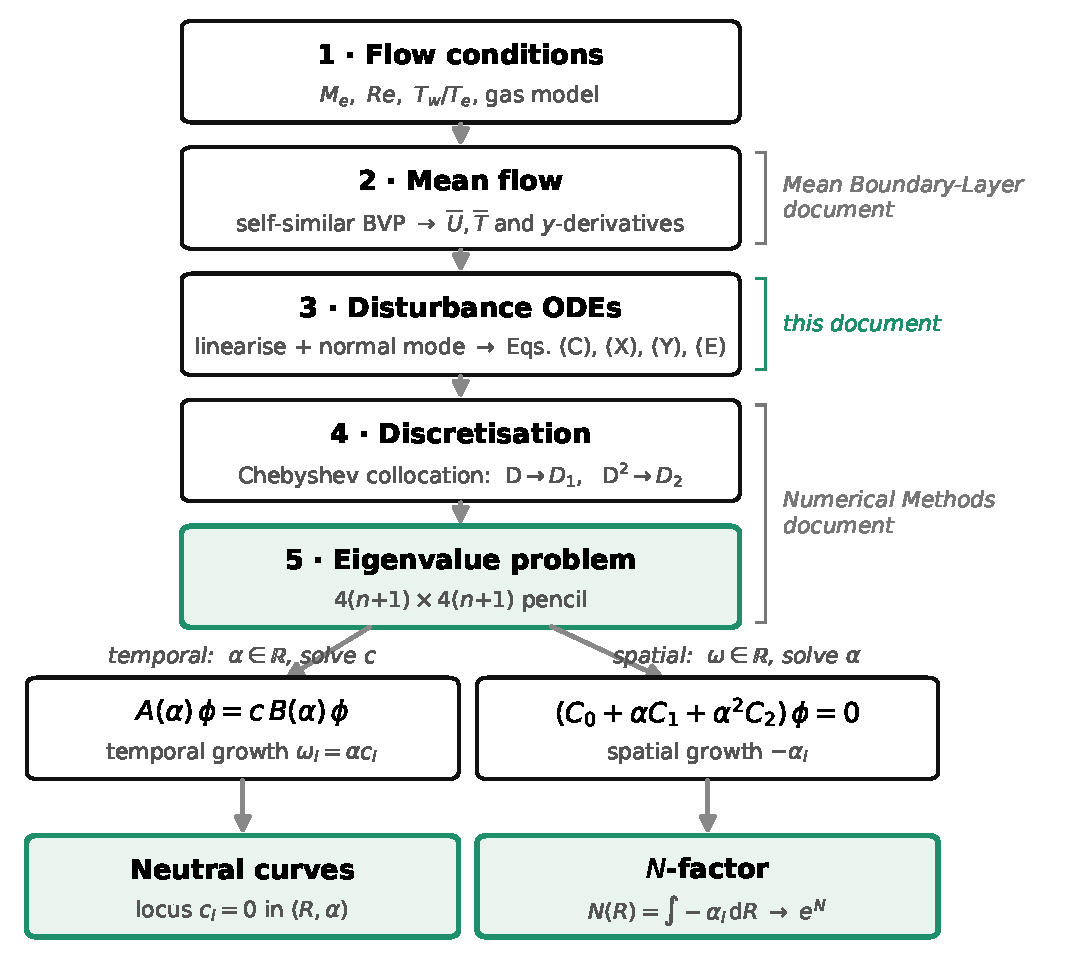
\includegraphics[width=0.72\linewidth]{fig_workflow.pdf}
  \caption{The complete LST computation in \texttt{pyMack}. Stages 1--2 are covered by the companion
  \emph{Mean Boundary-Layer} document, stage~3 by the present document, and stages 4--5 by the
  companion \emph{Numerical Methods} document; the two solution routes are temporal (fixed real
  $\alpha$, complex $c$) and spatial (fixed real $\omega$, complex $\alpha$).}\label{fig:workflow}
\end{figure}

\paragraph{Notation.} Overbars denote mean (base-flow) quantities; hats denote complex disturbance
amplitudes. The continuous wall-normal amplitude vector is $\hatq(y)=(\hatu,\hatv,\hatT,\hatp)$. A prime
on a mean quantity denotes $\D\equiv\mathrm d/\mathrm dy$; from Section~\ref{sec:operator} onward the
distinction between the continuous operator $\D$ and its discrete counterpart is made explicit.
\begin{center}\footnotesize
\renewcommand{\arraystretch}{1.18}
\begin{tabular}{@{}ll@{\hspace{1.4em}}ll@{}}
\toprule
\multicolumn{2}{@{}l}{\textbf{Base flow \& transport}} & \multicolumn{2}{l}{\textbf{Disturbance / eigenvalue}}\\
$\bar U,\bar T,\bar\rho{=}1/\bar T$ & mean velocity, temp., density & $\hatq$ & amplitude shape, Eq.~\eqref{eq:ansatz}\\
$\bar\mu,\bar\kappa$ & viscosity, conductivity & $\hatu,\hatv,\hatT,\hatp$ & velocity/temp./pressure amplitudes\\
$\Mae,\ \Ree,\ \mathit{Pr},\ \gamma$ & Mach, Reynolds, Prandtl, $c_p/c_v$ & $\alpha,\ \omega$ & wavenumber, frequency\\
$\nuR{=}1/(\Ree\bar\rho)$ & viscous prefactor & $c{=}\omega/\alpha$ & complex phase speed; $c_r,c_i$ its parts\\
$\mathcal C_\kappa,\mathcal C_d,\mathcal L_c$ & conduction/dissipation groups & $M_{\rm rel}$ & relative Mach number, \S\ref{sec:mechanisms}\\
\bottomrule
\end{tabular}
\end{center}

%=====================================================================
\section{Linearisation and the normal-mode ansatz}\label{sec:lin}
%=====================================================================
The flow is governed by the compressible Navier--Stokes equations, expressing conservation of mass,
momentum, and energy for a viscous, heat-conducting perfect gas \cite{white2006}:
\begin{align}
  \frac{\D\rho}{\D t}+\rho\,\nabla\!\cdot\!\mathbf u &= 0, &&\text{(mass)}\label{eq:ns-mass}\\
  \rho\frac{\D\mathbf u}{\D t} &= -\nabla p+\nabla\!\cdot\!\boldsymbol\tau, &&\text{(momentum)}\label{eq:ns-mom}\\
  \rho\,c_p\frac{\D T}{\D t} &= \frac{\D p}{\D t}+\nabla\!\cdot(\kappa\nabla T)+\Phi, &&\text{(energy)}\label{eq:ns-energy}\\
  p &= \rho R T, &&\text{(state)}\label{eq:ns-state}
\end{align}
where $\mathbf u=(u,v)$ is the velocity, $\rho$ the density, $T$ the temperature, $p$ the pressure,
$\mu$ the viscosity, $\kappa$ the conductivity, $c_p$ the specific heat, $R$ the gas constant,
$\D/\D t=\partial_t+\mathbf u\!\cdot\!\nabla$ the material derivative, $\boldsymbol\tau$ the Newtonian
viscous stress tensor, and $\Phi=\boldsymbol\tau\!:\!\nabla\mathbf u$ the dissipation function (both
linear in the velocity gradients). These are the same equations solved for the steady mean flow in the
companion document; they are applied here a second time, in linearised form, for the disturbance. The
reduction to ordinary differential equations proceeds in five steps.

\paragraph{Step 1: decomposition into mean and disturbance.} Each field is split as
\begin{equation}\label{eq:split}
  u=\bar U(y)+u',\ \ v=v',\ \ T=\bar T(y)+T',\ \ p=\bar p+p',\ \ \rho=\bar\rho(y)+\rho',\qquad
  |\cdot'|\ll|\bar\cdot|,
\end{equation}
with $\bar v=0$ for a parallel mean flow. The collection $q'=(u',v',T',p',\rho')$ is the disturbance.

\paragraph{Step 2: linearisation.} Substituting \eqref{eq:split} into
\eqref{eq:ns-mass}--\eqref{eq:ns-state}, the mean satisfies the equations by itself and cancels; terms
quadratic in the primed quantities are dropped. The remaining equations are linear in $q'$ with
coefficients constructed from the known mean profiles.

\paragraph{Step 3: parallel-flow assumption.} The boundary layer grows slowly, so locally
$\bar q=\bar q(y)$ only and the coefficients depend on $y$ alone. This neglects the $O(1/R)$ streamwise
growth of the mean flow and of the eigenfunction; the systematic remedy, retaining that slow
$x$-variation, is the parabolised stability equations \cite{herbert1997} (cf.\
Section~\ref{sec:scope}).

\paragraph{Step 4: normal-mode ansatz.} The disturbance is represented as a single travelling wave,
\begin{equation}\label{eq:ansatz}
  q'(x,y,t)=\hatq(y)\,e^{\imag(\alpha x-\omega t)},\qquad \hatq=(\hatu,\hatv,\hatT,\hatp)^{\mathsf T},
\end{equation}
with $\alpha$ the streamwise wavenumber, $\omega$ the frequency, and $c=\omega/\alpha$ the complex phase
speed. Substitution replaces $\partial_x\mapsto\imag\alpha$, $\partial_t\mapsto-\imag\omega$, and
$\partial_y\mapsto\D$, collapsing the linear PDEs to coupled ODEs in $y$
(Figure~\ref{fig:ansatz}). The spanwise wavenumber is set to zero ($\beta=0$); a general oblique wave
$\propto e^{\imag(\alpha x+\beta z-\omega t)}$ propagates at angle $\psi=\arctan(\beta/\alpha)$, and
since Squire's theorem does not carry over to compressible flow, the first mode is most unstable oblique
($\psi\sim55^\circ$) while the second mode is most unstable at $\psi=0$ \cite{mack1984}. The
consequences of the two-dimensional restriction are recorded in Section~\ref{sec:scope}.

\paragraph{Step 5: elimination of density.} The linearised equation of state gives
\begin{equation}\label{eq:state-lin}
  \frac{\rho'}{\bar\rho}=\gamma\Mae^2\,\hatp-\frac{\hatT}{\bar T},
\end{equation}
which removes $\rho'$ from the system. Four amplitude fields remain, $\hatu,\hatv,\hatT,\hatp$, with
$\hatp$ scaled by $\rho_eU_e^2$ (so that $\gamma\Mae^2\hatp=p'/p_e$).

\paragraph{A worked linearisation.} To make the mechanics explicit, consider mass conservation
\eqref{eq:ns-mass}, $\partial_t\rho+\nabla\!\cdot(\rho\mathbf u)=0$. Inserting \eqref{eq:split}, the
steady mean satisfies $\partial_x(\bar\rho\bar U)=0$ and cancels; retaining only terms linear in the
primed quantities,
\begin{equation}
  \partial_t\rho'+\bar U\,\partial_x\rho'+\bar\rho\,\partial_x u'+\partial_y(\bar\rho v')=0 .
\end{equation}
Applying the ansatz \eqref{eq:ansatz} ($\partial_t\to-\imag\alpha c$, $\partial_x\to\imag\alpha$,
$\partial_y\to\D$), substituting $\rho'$ from \eqref{eq:state-lin}, collecting terms, and dividing by
$\bar\rho$ yields exactly Eq.~\eqref{eq:cont} below. The remaining three equations follow by the
identical procedure applied to \eqref{eq:ns-mom}--\eqref{eq:ns-energy}; the algebra is mechanical but
lengthy, and only the result is printed.

\begin{figure}[H]\centering
  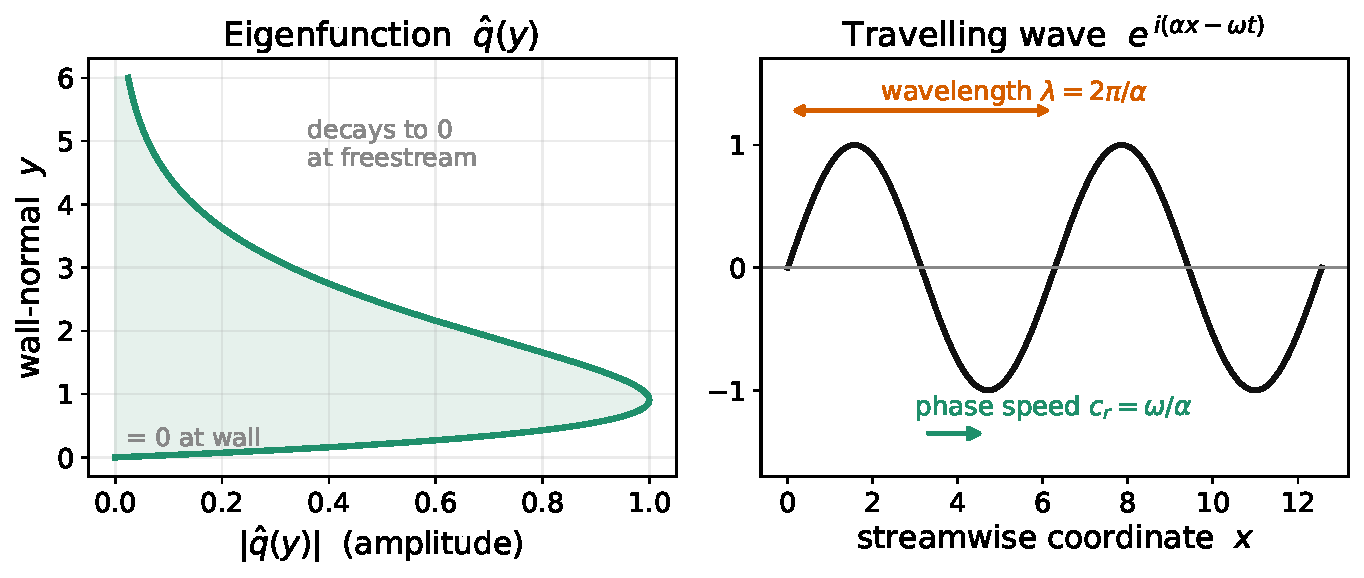
\includegraphics[width=0.92\linewidth]{fig_ansatz.pdf}
  \caption{The ansatz \eqref{eq:ansatz} factorises a disturbance
  $q'=\hatq(y)\,e^{\imag(\alpha x-\omega t)}$ into a wall-normal \emph{shape} $\hatq(y)$ (left; the
  eigenfunction, zero at the wall and decaying at the edge) and a travelling wave in $x$ (right; wavelength
  $2\pi/\alpha$, phase speed $c_r=\Real(c)$).}\label{fig:ansatz}
\end{figure}

%=====================================================================
\section{The four disturbance equations}\label{sec:eqs}
%=====================================================================
The linearised system consists of four coupled ODEs in $y$ for $\hatu,\hatv,\hatT,\hatp$: continuity
(with the equation of state folded in through \eqref{eq:state-lin}), streamwise and wall-normal
momentum, and energy. Fixing one of $\alpha$ or $\omega$ real leaves the other (through $c$ or
$\alpha$) as the eigenvalue. Every overbarred quantity is a known base-flow coefficient; all transport
derivatives ($\mathrm d\mu/\mathrm dT$, $\mathrm d\kappa/\mathrm dT$, \dots) are evaluated at the local
mean temperature $\bar T(y)$ and are therefore known functions of $y$. The form below, assembled in
\texttt{pymack/temporal\_solver.py}, follows \"Ozgen \& K{\i}rcal{\i} \cite{ozgen2008}; it is
equivalent to the canonical compressible stability equations of Mack \cite{mack1984} and Malik
\cite{malik1990} restricted to two dimensions. Momentum and energy are divided by $\bar\rho$, and the
viscous prefactor is written $\nuR\equiv1/(\Ree\,\bar\rho)$; every $\bar\rho$ is the base-flow density
$\bar\rho(y)=1/\bar T(y)$, uniformly inside $\nuR$, $\mathcal C_\kappa$, and $\mathcal C_d$.

\paragraph{(C) Continuity $+$ equation of state.}
\begin{equation}\label{eq:cont}
  \imag\alpha\hatu+\D\hatv-\frac{\bar T'}{\bar T}\hatv
  +\imag\alpha(\bar U-c)\Big(\gamma\Mae^2\hatp-\frac{\hatT}{\bar T}\Big)=0 .
\end{equation}

\paragraph{(X) Streamwise momentum.}
\begin{equation}\label{eq:xmom}
\begin{aligned}
  \imag\alpha(\bar U-c)\hatu+\bar U'\hatv+\imag\alpha\bar\rho^{-1}\hatp
  =\nuR\Big[&\bar\mu\big(\D^2-\tfrac43\alpha^2\big)\hatu+\bar\mu'\D\hatu
     +\imag\alpha\big(\tfrac13\bar\mu\D+\bar\mu'\big)\hatv\\
   &+\tfrac{\mathrm d\mu}{\mathrm dT}\big(\bar U''+\bar U'\D\big)\hatT
     +\tfrac{\mathrm d^2\mu}{\mathrm dT^2}\bar U'\bar T'\hatT\Big] .
\end{aligned}
\end{equation}

\paragraph{(Y) Wall-normal momentum.}
\begin{equation}\label{eq:ymom}
\begin{aligned}
  \imag\alpha(\bar U-c)\hatv+\bar\rho^{-1}\D\hatp
  =\nuR\Big[&\bar\mu\big(\tfrac43\D^2-\alpha^2\big)\hatv+\tfrac43\bar\mu'\D\hatv
   +\imag\alpha\big(\tfrac13\bar\mu\D-\tfrac23\bar\mu'\big)\hatu
   +\imag\alpha\tfrac{\mathrm d\mu}{\mathrm dT}\bar U'\hatT\Big] .
\end{aligned}
\end{equation}

\paragraph{(E) Energy (temperature).}
\begin{equation}\label{eq:energy}
  \imag\alpha(\bar U-c)\hatT+\bar T'\hatv+(\gamma-1)\bar\rho^{-1}\big(\imag\alpha\hatu+\D\hatv\big)
  =\mathcal C_\kappa\mathcal L_c\hatT
   +\mathcal C_d\Big[2\bar\mu\bar U'\big(\D\hatu+\imag\alpha\hatv\big)
     +\tfrac{\mathrm d\mu}{\mathrm dT}\big(\bar U'\big)^2\hatT\Big],
\end{equation}
\begin{equation}\label{eq:groups}
  \mathcal L_c=\D^2-\alpha^2
   +\tfrac1{\bar\kappa}\tfrac{\mathrm d\kappa}{\mathrm dT}\big(2\bar T'\D+\bar T''\big)
   +\tfrac1{\bar\kappa}\tfrac{\mathrm d^2\kappa}{\mathrm dT^2}\big(\bar T'\big)^2,\quad
  \mathcal C_\kappa=\frac{\gamma\bar\mu}{\mathit{Pr}\,\Ree\,\bar\rho},\quad
  \mathcal C_d=\frac{\gamma(\gamma-1)\Mae^2}{\Ree\,\bar\rho}.
\end{equation}

\paragraph{Structure of the equations.} The following observations locate the physics in
\eqref{eq:cont}--\eqref{eq:energy}:
\begin{itemize}[nosep,leftmargin=1.6em]
  \item $\imag\alpha(\bar U-c)$ is convection by the mean flow relative to the wave; it vanishes at the
        \emph{critical layer} $\bar U=c_r$, where the inviscid form of the equations becomes singular,
        which is why that layer governs much of the instability physics \cite{mack1984}.
  \item $\D,\D^2$ are wall-normal derivatives; the $-\alpha^2$ terms arise from
        $\partial_x^2\mapsto-\alpha^2$.
  \item The $\nuR=1/(\Ree\bar\rho)$ terms are viscous; the factors $\tfrac43,\tfrac13$ correspond to the
        Stokes hypothesis for the bulk viscosity (the companion \emph{Numerical Methods} document
        generalises this to a ratio $\lambda/\mu=1.2$ in the spatial closure).
  \item $(\gamma-1)\bar\rho^{-1}(\imag\alpha\hatu+\D\hatv)$ in \eqref{eq:energy} is pressure
        (dilatation) work: $\imag\alpha\hatu+\D\hatv$ is the linearised velocity divergence, so
        compression or expansion of a fluid parcel heats or cools it, coupling the velocity field back
        into the temperature equation.
  \item The $\mathrm d\mu/\mathrm dT$, $\mathrm d\kappa/\mathrm dT$ terms represent
        temperature-dependent transport, essential at hypersonic conditions.
  \item $\mathcal C_\kappa\mathcal L_c\hatT$ is heat conduction; $\mathcal C_d[\cdots]$ is viscous
        dissipation.
\end{itemize}

%=====================================================================
\section{Operator form and the discretised derivative}\label{sec:operator}
%=====================================================================
Equations \eqref{eq:cont}--\eqref{eq:energy} are linear both in the amplitude vector
$\hatq=(\hatu,\hatv,\hatT,\hatp)^{\mathsf T}$ and in the eigenvalue, and every derivative they contain
is of at most second order. They can therefore be collected into the single operator statement
\begin{equation}\label{eq:pencil}
  \mathsf L(\alpha;y,\D)\,\hatq \;=\; c\,\mathsf M(\alpha;y)\,\hatq,
  \qquad
  \mathsf L=\mathsf A_2(y)\,\D^2+\mathsf A_1(\alpha;y)\,\D+\mathsf A_0(\alpha;y),
\end{equation}
with rows ordered (C, X, Y, E) and columns ordered $(\hatu,\hatv,\hatT,\hatp)$. Two structural facts
make \eqref{eq:pencil} particularly convenient for what follows.

First, the eigenvalue $c$ enters \eqref{eq:cont}--\eqref{eq:energy} \emph{only} through the convective
factor $\imag\alpha(\bar U-c)$. The right-hand operator $\mathsf M$ is therefore purely algebraic,
containing no derivatives, and can be written down at once:
\begin{equation}\label{eq:Mmat}
  \mathsf M(\alpha;y)=\imag\alpha
  \begin{pmatrix}
    0 & 0 & -1/\bar T & \gamma\Mae^2\\
    1 & 0 & 0 & 0\\
    0 & 1 & 0 & 0\\
    0 & 0 & 1 & 0
  \end{pmatrix}.
\end{equation}

Second, only three terms in the entire system carry $\D^2$: the viscous diffusion of $\hatu$ and
$\hatv$ in \eqref{eq:xmom}--\eqref{eq:ymom} and the heat conduction of $\hatT$ in \eqref{eq:energy}.
The second-order coefficient matrix is therefore sparse:
\begin{equation}\label{eq:A2mat}
  \mathsf A_2(y)=
  \begin{pmatrix}
    0 & 0 & 0 & 0\\
    -\nuR\bar\mu & 0 & 0 & 0\\
    0 & -\tfrac43\nuR\bar\mu & 0 & 0\\
    0 & 0 & -\mathcal C_\kappa & 0
  \end{pmatrix},
\end{equation}
where the signs follow from moving the right-hand sides of \eqref{eq:xmom}--\eqref{eq:energy} to the
left. The pressure amplitude $\hatp$ is never differentiated twice, so its column in $\mathsf A_2$ is
empty, reflecting the absence of a pressure diffusion mechanism. The first- and zeroth-order
matrices $\mathsf A_1$ and $\mathsf A_0$ are read off from \eqref{eq:cont}--\eqref{eq:energy} in the
same manner; their entries are the convective, pressure-gradient, mean-shear, and
transport-derivative coefficients, and they are assembled term by term in
\texttt{pymack/temporal\_solver.py}.

\paragraph{Temporal and spatial problems.} Equation \eqref{eq:pencil} supports the two standard
closures. Fixing $\alpha\in\mathbb R$ leaves $c$ as the eigenvalue of a \emph{linear} operator
pencil; this is the temporal problem. Fixing $\omega\in\mathbb R$ instead and regrouping the same equations
by powers of $\alpha$ gives
\begin{equation}\label{eq:spatial}
  \big(\mathsf C_0(\omega;y,\D)+\alpha\,\mathsf C_1(\omega;y,\D)+\alpha^2\,\mathsf C_2(y)\big)\hatq=0,
\end{equation}
a \emph{quadratic} pencil in $\alpha$; this is the spatial problem, reduced to linear form by
companion linearisation in the companion \emph{Numerical Methods} document.

\paragraph{The discretised derivative operator.} Up to this point $\D$ has denoted the continuous
derivative $\mathrm d/\mathrm dy$ acting on smooth functions. Numerical solution replaces it by a
discrete differentiation operator: the amplitudes are sampled on a collocation grid
$\{y_j\}_{j=0}^{n}$, and
\begin{equation}\label{eq:Ddiscrete}
  \D\;\longrightarrow\;D_1,\qquad \D^2\;\longrightarrow\;D_2,\qquad
  D_1,D_2\in\mathbb R^{(n+1)\times(n+1)},
\end{equation}
where $D_1$, $D_2$ are the Chebyshev collocation differentiation matrices mapped to the physical
domain, the natural discretisation for boundary-layer eigenvalue problems
\cite{orszag1971,malik1990}. Under \eqref{eq:Ddiscrete} each mean-flow coefficient becomes a diagonal
matrix, each entry of $\mathsf A_2,\mathsf A_1,\mathsf A_0,\mathsf M$ becomes an
$(n{+}1)\times(n{+}1)$ block, and the four sampled amplitudes are stacked into a single vector
$\boldsymbol\phi=(\hatu;\hatv;\hatT;\hatp)\in\mathbb C^{4(n+1)}$. The operator statement
\eqref{eq:pencil} then becomes the finite-dimensional generalised eigenvalue problem
\begin{equation}\label{eq:gevp}
  \boxed{\;A(\alpha)\,\boldsymbol\phi=c\,B(\alpha)\,\boldsymbol\phi\;}\qquad
  A,B\in\mathbb C^{4(n+1)\times4(n+1)},
\end{equation}
which is the object \texttt{pymack/temporal\_solver.py} assembles and solves.

\paragraph{Anatomy of the discrete problem.} Equation \eqref{eq:gevp} deserves to be read carefully:
it is the computational atom of the entire framework, and each of its symbols has a definite meaning
inherited from the derivation above.

The matrix $A(\alpha)$ is the discretisation of the left-hand operator $\mathsf L$ of
\eqref{eq:pencil}: it carries \emph{all of the eigenvalue-independent physics}, namely mean-flow
convection $\imag\alpha\bar U$, the pressure gradient, mean-shear production, viscous diffusion, heat
conduction, and the dilatational coupling, evaluated at the chosen wavenumber $\alpha$. The matrix
$B(\alpha)$ is the discretisation of the algebraic operator $\mathsf M$ of \eqref{eq:Mmat}: it marks
exactly \emph{where the eigenvalue enters} the equations, which, since $-\imag\omega=-\imag\alpha c$,
is precisely where the time derivative acted before the ansatz \eqref{eq:ansatz}. Both inherit the
$4\times4$ block structure of the operator form: with $i,j$ ranging over the rows (C,\,X,\,Y,\,E) and
the columns $(\hatu,\hatv,\hatT,\hatp)$,
\begin{equation}\label{eq:blocks}
  A_{ij}(\alpha)=\Lambda\big([\mathsf A_2]_{ij}\big)\,D_2+\Lambda\big([\mathsf A_1]_{ij}\big)\,D_1
  +\Lambda\big([\mathsf A_0]_{ij}\big),
  \qquad
  B_{ij}(\alpha)=\Lambda\big([\mathsf M]_{ij}\big),
\end{equation}
where $\Lambda(f)=\mathrm{diag}\big(f(y_0),\dots,f(y_n)\big)$ places a known coefficient function on
the grid. Every entry of $A$ and $B$ is therefore an $(n{+}1)\times(n{+}1)$ block built from exactly
three ingredients: the differentiation matrices $D_1,D_2$, diagonal samples of mean-flow profiles, and
the scalars $\alpha$, $\Mae$, $\Ree$. The eigenvector
$\boldsymbol\phi=(\hatu;\hatv;\hatT;\hatp)$ stacks the four amplitude profiles sampled on the same
grid: it \emph{is} the eigenfunction $\hatq(y)$ of \eqref{eq:pencil}, represented by its values at
the collocation points.

A single solve of \eqref{eq:gevp} returns the full discrete spectrum: of order $4(n{+}1)$ eigenpairs
$(c,\boldsymbol\phi)$. Each eigenpair is a candidate normal mode of the boundary layer at the given
$(\Mae,\Ree,\alpha)$: the real part $c_r$ is its phase speed as a fraction of $U_e$; the imaginary
part sets its temporal growth rate $\omega_i=\alpha c_i$, so $c_i>0$ identifies an amplifying wave,
$c_i<0$ a damped one, and $c_i=0$ a neutral one; and the four segments of $\boldsymbol\phi$ give the
wave's internal structure: the velocity, temperature, and pressure amplitude profiles across the
layer (a wall-peaked $|\hatp|$, for instance, signals a second mode). Only a handful of these
eigenpairs are physical \emph{discrete} modes; the remainder approximate the continuous spectra or
are numerical artifacts. In particular, the boundary-condition rows carry no eigenvalue and leave
zero rows in $B$, so $B$ is singular and the pencil must be solved in generalised (QZ) form,
producing spurious infinite eigenvalues that are discarded. The identification of the physical modes
within this spectrum is treated in the companion \emph{Numerical Methods} document.

Everything the framework ultimately produces is assembled from repeated solves of \eqref{eq:gevp}:
one solve interrogates one point of the parameter space $(\Mae,\Ree,\alpha)$, a sweep of solves
traces the growth rate across the $(R,\alpha)$ plane, the zero level set $c_i=0$ of that sweep is the
neutral curve, and the integral of the growth rate along frequency lines is the $N$-factor. The
construction of $D_1,D_2$, the wall-clustering domain map, the boundary-condition rows, the solution
of \eqref{eq:gevp} and of the spatial pencil \eqref{eq:spatial}, and the classification of the
resulting spectrum are the subject of the companion \emph{Numerical Methods} document.

%=====================================================================
\section{Physical character of the instability modes}\label{sec:mechanisms}
%=====================================================================
The disturbance equations admit discrete eigenmodes; a temporal solve returns a complex phase speed
such as $c=0.930+0.0200\imag$. This section summarises the physics behind the standard mode labels, so
that such a number identifies a definite wave.

\paragraph{First (Tollmien--Schlichting) mode.} At low speed the first mode is a viscous instability
($c_r\approx0.3$--$0.6$): viscosity introduces a phase lag between $u'$ and $v'$ near the wall, so the
Reynolds stress $-\bar\rho\,\overline{u'v'}$ no longer averages to zero and extracts energy from the
mean shear. As the Mach number rises, compressibility creates a generalised inflection point (below)
and the first mode becomes increasingly inviscid and inflectional, with viscosity then often acting to
stabilise; it is the dominant instability only up to $\Mae\approx4$ \cite{mack1984}.

\paragraph{Second (Mack) mode.} Above $\Mae\approx4$ a second, usually stronger, instability appears:
an acoustic wave trapped between the wall and the relative sonic line, reflecting within a near-wall
acoustic waveguide \cite{mack1984,fedorov2011}. This interpretation accounts for its principal
properties:
\begin{itemize}[nosep,leftmargin=1.6em]
  \item its phase speed is $c_r\approx1-1/\Mae$, the limiting value at which the wave is sonic relative
        to the edge flow, which is why the spatial-solve shift target $\alpha_0=\omega/(1-1/\Mae)$ is
        effective; the realised $c_r$ sits somewhat above this and varies along the branch ($0.93$
        against $1-1/6=0.83$ for a representative $\Mae=6$ mode);
  \item it is frequency-tuned: as in any resonator the wavelength is set by the cavity thickness, so
        the most-amplified wavelength is ${\sim}2\delta$ and the frequency scales as
        $f\sim U_e/2\delta$, rising as the layer thins downstream;
  \item its eigenfunction has a wall-peaked pressure amplitude, the acoustic field of the waveguide.
\end{itemize}

\paragraph{The organising quantity: relative Mach number.} Both mechanisms are organised by the
relative Mach number
\begin{equation}\label{eq:mrel}
  M_{\rm rel}(y)=\frac{\bar U(y)-c_r}{\bar a(y)},\qquad \bar a=\frac{\sqrt{\bar T}}{\Mae},
\end{equation}
with $\bar a$ the local sound speed. The critical layer is the height at which $M_{\rm rel}=0$, i.e.\
$\bar U=c_r$, where the eigenfunction typically peaks and the convective factor
$\imag\alpha(\bar U-c)$ in \eqref{eq:cont}--\eqref{eq:energy} vanishes; the relative sonic line is
$|M_{\rm rel}|=1$; and the second-mode acoustic waveguide is the near-wall region in which
$|M_{\rm rel}|>1$.

\paragraph{The generalised inflection point.} By Rayleigh's theorem an inviscid incompressible shear
flow requires a velocity inflection point ($\bar U''=0$) for instability. Lees \& Lin
\cite{leeslin1946} generalised this to compressible flow: the necessary condition for the inviscid
first mode is a \emph{generalised inflection point}, $(\bar\rho\,\bar U')'=0$. Aerodynamic heating
places a hot, low-density layer near the wall and pushes that point up into the layer, giving
compressible boundary layers a robust inviscid first-mode instability that low-speed layers lack. The
second mode requires no inflection point; its existence condition is instead the relative-supersonic
region $|M_{\rm rel}|>1$ above.

\paragraph{The wall-cooling reversal.} Cooling the wall stabilises the first mode (it weakens the
near-wall viscous mechanism) but destabilises the second (it thickens the relative-supersonic region
and raises the tuned frequency) \cite{mack1984}. Cold-walled hypersonic vehicles are therefore
second-mode dominated, which is why the solver carries an isothermal-wall option.

\paragraph{Phase and group velocity.} $c_r$ is the phase speed; energy propagates at the group
velocity $c_g=\mathrm d\omega_r/\mathrm d\alpha_r$, and it is $c_g$ that rigorously links temporal to
spatial growth \cite{gaster1962} (used when the companion \emph{Numerical Methods} document converts
between the two formulations).

\medskip
\noindent The following comparison places any computed eigenvalue at a glance:
\begin{center}\small
\renewcommand{\arraystretch}{1.2}
\begin{tabular}{@{}>{\raggedright\arraybackslash}p{3.1cm}>{\raggedright\arraybackslash}p{5.1cm}>{\raggedright\arraybackslash}p{5.1cm}@{}}
\toprule
 & \textbf{First (TS) mode} & \textbf{Second (Mack) mode} \\
\midrule
mechanism & viscous (low speed) $\to$ inviscid inflectional (high speed) & trapped acoustic wave (wall--sonic line) \\
phase speed $c_r$ & $0.3$--$0.6$ & $\approx 1-1/\Mae$ \\
dominant when & low speed, $\Mae\lesssim4$ & high speed, $\Mae\gtrsim4$ \\
frequency & broadband & tuned, $f\sim U_e/2\delta$ \\
existence criterion & generalised inflection point \cite{leeslin1946} & relative-supersonic region, $|M_{\rm rel}|>1$ \\
wall cooling & stabilises & destabilises \\
most-unstable wave & oblique (3D) & 2D ($\psi=0$) \\
\bottomrule
\end{tabular}
\end{center}

%=====================================================================
\section{Assumptions and range of validity}\label{sec:scope}
%=====================================================================
The equations derived above are the two-dimensional, parallel-flow, modal disturbance equations. Four
idealisations bound their interpretation:
\begin{enumerate}[nosep,leftmargin=1.9em]
  \item \textbf{Parallel flow.} Setting $\bar v=0$ with $y$-only coefficients (Step~3) neglects the
        $O(1/R)$ streamwise growth of the layer; the systematic remedy is the parabolised stability
        equations, which march the disturbance downstream retaining the slow $x$-variation
        \cite{herbert1997}.
  \item \textbf{Two-dimensionality.} The ansatz takes $\beta=0$ (Step~4). The most-unstable first mode
        is oblique ($\psi\sim55^\circ$; Squire's theorem does not hold under compressibility
        \cite{mack1984}), so two-dimensional first-mode growth is a lower bound; the second mode is
        most unstable at $\psi=0$, so the two-dimensional result is its physical maximum.
  \item \textbf{Modal analysis.} Eigenvalues describe asymptotic exponential growth; the non-normal
        operator also permits transient (algebraic) growth that modal analysis misses, relevant to
        bypass and blunt-body transition paths \cite{schmid2001}.
  \item \textbf{Receptivity and $e^N$.} LST provides the amplification \emph{ratio}
        $A(R)/A(R_0)=e^N$, not the initial amplitude $A(R_0)$; determining that amplitude is the
        separate receptivity problem, and the $e^N$ method is an environment-dependent correlation
        rather than a first-principles criterion \cite{vaningen1956,fedorov2011}.
\end{enumerate}
None of these affect the equations themselves; they delimit their range of validity. A strong second
mode is captured faithfully by the two-dimensional modal equations derived here, which is why they are
the workhorse of hypersonic transition prediction \cite{mack1984,fedorov2011}. With the system
\eqref{eq:cont}--\eqref{eq:energy} in operator form \eqref{eq:pencil} and its discrete counterpart
\eqref{eq:gevp} identified, the construction and solution of the matrix problem proceed in the
companion \emph{Numerical Methods} document.

\begin{thebibliography}{99}
\bibitem{mack1984} L.~M. Mack, ``Boundary-layer linear stability theory,'' AGARD Report No.~709,
  \emph{Special Course on Stability and Transition of Laminar Flow}, 1984.
\bibitem{white2006} F.~M. White, \emph{Viscous Fluid Flow}, 3rd ed., McGraw--Hill, New York, 2006.
\bibitem{ozgen2008} S.~\"Ozgen and S.~A. K{\i}rcal{\i}, ``Linear stability analysis in compressible,
  flat-plate boundary layers,'' \emph{Theoretical and Computational Fluid Dynamics}, Vol.~22, 2008,
  pp.~1--20.
\bibitem{malik1990} M.~R. Malik, ``Numerical methods for hypersonic boundary layer stability,''
  \emph{Journal of Computational Physics}, Vol.~86, No.~2, 1990, pp.~376--413.
\bibitem{orszag1971} S.~A. Orszag, ``Accurate solution of the Orr--Sommerfeld stability equation,''
  \emph{Journal of Fluid Mechanics}, Vol.~50, No.~4, 1971, pp.~689--703.
\bibitem{leeslin1946} L.~Lees and C.~C. Lin, ``Investigation of the stability of the laminar boundary
  layer in a compressible fluid,'' NACA Technical Note No.~1115, 1946.
\bibitem{gaster1962} M.~Gaster, ``A note on the relation between temporally-increasing and
  spatially-increasing disturbances in hydrodynamic stability,'' \emph{Journal of Fluid Mechanics},
  Vol.~14, 1962, pp.~222--224.
\bibitem{herbert1997} T.~Herbert, ``Parabolized stability equations,'' \emph{Annual Review of Fluid
  Mechanics}, Vol.~29, 1997, pp.~245--283.
\bibitem{schmid2001} P.~J. Schmid and D.~S. Henningson, \emph{Stability and Transition in Shear
  Flows}, Springer, New York, 2001.
\bibitem{vaningen1956} J.~L. van Ingen, ``A suggested semi-empirical method for the calculation of the
  boundary layer transition region,'' Report VTH-74, Delft University of Technology, 1956.
\bibitem{fedorov2011} A.~Fedorov, ``Transition and stability of high-speed boundary layers,''
  \emph{Annual Review of Fluid Mechanics}, Vol.~43, 2011, pp.~79--95.
\end{thebibliography}

\end{document}
